\chapter{经典逻辑上的抽象机 $\amlh$}

\section{原理概览} \label{Sec.Overview}

在定理证明器上以经典逻辑预先定义一系列基元函数作为抽象机的基元指令集,
这些基元函数的正确性并非被证明而是作为公理。
基于这些基元函数以$\lambda$演算构建起抽象机。
或是更严谨地说抽象机是在简单类型$\lambda$演算这一个形式系统上
引入一系列作为公理规则的基元函数,
并削除一些功能以将此新的形式系统上的运算限制在基元函数的组合。
抽象机上的程序是这些基元函数的组合。
一些常用的组合可以被保存,作为函数库的形式被之后用户使用。
那么抽象机上的编程就是对基元函数的组合以及这些组合的组合。

这一抽象机是一种形式系统,本文使用记号 $\amlh$ 表示。

基元函数被巧妙的设定,尽可能基层的同时保持良好的数学亲和性。
基元函数即是基元指令,令基元指令集尽可能接近目标编译平台,尽可能的基础,
那么程序的基元指令表达本身就足够接近目标编译平台的汇编表达,
就可以作为编译的中间表达(IR)而输出并由外部程序进行
简单的处理就能编译到目标平台。

那么$\amlh$上的抽象程序到中间表达的编译过程实质就是将抽象程序完全展开到
基元函数表达。这种展开是在定理证明器上进行的等价变换,
编译正确性是有保障的到中间表达级别的。
而外部程序对中间表达到目标平台的编译是固定的且尽可能的简单,
未来可以对这一最后的编译过程进行额外的验证,就可以将编译保障的范围延伸。

这些基元指令虽然简单但可以构造一门编程语言与一系列的理论工具辅助,再
在定理证明器上实现这一系列辅助包括各种半自动的证明策略与分析工具,
最后在外部构建一个完整的接口壳层将一切工具与接口统一起来。
以此提供非常有效的程序开发支持能力。
这么做是可行的,因为传统软件工程就是这样一层层的抽象与辅助而将
用户以编程语言为格式而以源代码为载体承载的抽象思维与执行逻辑一步步翻译转换
最终生成对应的目标平台上机器编码的可执行程序。
即本质上是要模仿传统软件工程的体系而在数理的范畴内再实现一遍。

而在数理的抽象上进行软件工程也意味着大量的改变。

直接使用$\lambda$演算构建抽象机的主要困难有两点。
第一点是系统状态相关的建模,现实的计算机中有大量的系统状态,
而$\lambda$演算本身是无状态的。通用的方案是使用状态机模型而不是直接用$\lambda$演算,
但本工作是从头基于抽象数理设计软件开发故而可以有新的思路。
第二点是线程,状态机模型上线程可以有清晰的概念,而在$\lambda$演算中则并没有。
事实上数理思维中并没有“执行”的概念,就更没有由一系列“执行”按时间线索先后联系在一起构成的
线程。这两点通向相同的解决道路。

数理思维中没有线程,本工作认为,这是数理的一种优势。
$\amlh$不显示地区分线程或是要求用户显示地编写线程与线程操作,相反,既然
现在大量的软件工程实践揭示了并行编程的价值,就在一开始将$\amlh$构造成一个内在并行的系统。
即,$\amlh$上的操作如同数学操作是自然地并行的,串行仅当数值计算上或是逻辑上的依赖时
才会发生。如果操作$A$数值上依赖另一个操作$B$,即$A$的执行需要$B$的结果,
则由$B$到$A$的执行是串行的;
如果操作$A$逻辑上需要等待操作$B$完成后在进行,则需要用户显示地编写状态依赖后可以串行执行;
如果操作$A$和$B$间既没有计算依赖又没有状态依赖,则$A$与$B$是并行执行的。
依赖关系的存否决定并行还是串行,依赖关系的偏序方向决定串行的执行次序。
两个线程是否可以合法地并行,又取决于各自对系统资源的访问。

本工作抽象一切状态为系统资源。
在无状态即没有系统资源的情况下,只有数值依赖;
对于系统资源的访问,可以是数值依赖也可以是状态依赖。
$\amlh$ 是一种并行读取互斥写入(Concurrent Read Exclusive Write, CREW)模型,
即允许多个线程对同一个资源的同时读取却只允许同一时刻一个线程写入资源。
这里的写入与读取不需要是真正的写入或读取,理解为可并行的操作与互斥操作也许更好。
两个线程的并行是否合法即是对资源的访问是否满足CREW。
系统资源与依赖,这两个问题很相关,将在\ref{Sec.hisFlow}节的历史流模型中详细论述。

另外值得注意的,至今为止所说的并行并不要求编译结果也严格地遵守并行。
串行的程序很难并行执行而并行的程序是很容易串行执行的。
$\amlh$上的软件开发从设计到编写再到最后编译出中间表达是始终保持并行的,
但对中间表达最后到目标平台的编译可以根据具体实现自由地选择串行或者部分并行。


%有助于读者直观地感受,尽管其中一些无法绕过的概念与引理尚未给出。
%这些主要是系统状态相关的历史流理论,会在下一节给出论述,而现在将暂时搁置。

\section{$\amlh$的形式定义}

接下来本文一步步给出$\amlh$的形式定义。
首先是基于$\lamst$的且无状态纯粹数值计算的抽象机$\aml$,
然后将$\aml$实现在HOL定理证明器的HOL逻辑上,
$\aml$在HOL上的实现根据抽象级别的高低有两个版本,
粗粒度抽象机$\amlhC$与细粒度抽象机$\amlhF$,最后几节将分别论述其实现。

\section{无状态$\aml$的形式定义}

\begin{defin}[$\aml$] 基于定义\ref{Def.slam},$\aml$是$\lamst$的应用。
\begin{enumerate}
  \item 设定类型变量集
  \[ U_{\mathrm{A}} = \{ \mathrm{phenomenon} \} \]
  即$\aml$的类型变量集只有一个类型变量 $\mathrm{phenomenon}$。
  因 $\mathrm{phenomenon}$ 过长在以下的论述中将其简写为 $\mathrm{ph}$。
  根据公式\ref{Pi}求得对应的
    \[\Pi_\mathrm{A} \Coloneqq U_\mathrm{A} \mbar
        (\Pi_\mathrm{A} \rightarrow \Pi_\mathrm{A})\]
\item 定义字符串集合 $Const_\mathrm{V}$ 表示常量符号。

    \begin{equation}
    Const_\mathrm{V} = \{ \mathbf{Const}\ x\ b \mbar x, y \in \mathbb{N} \land x < 2^y \}
    \end{equation}
  且 $Const_\mathrm{V}$ 不与 $V$ 重合,即 $Const_\mathrm{V} \cap V = \emptyset$。
  定义常量集$Const$ 为满足如下语法的字符串集合。
        \[ Const \Coloneqq Const_\mathrm{V} : \mathrm{phenomenon} \]
  字符串 $\mathbf{Const}\ x\ b : \mathrm{phenomenon}$ 表示以$b$个二进制位表示的数值 $x$。
\item 定义一个可自由设定的有限字符串集合 $P_\mathrm{V}$ 为基元指令的符号集,
    且 $P_\mathrm{V}$ 不与 $V$ 或$Const_\mathrm{V}$重合。
    定义 $P_\mathrm{V}$ 到 $\Pi$ 的函数 $\mathcal{T}$ 为各个基元指令的类型。
    定义基元指令集$P$。
    \begin{equation}
    P = \{x:\mathcal{T}(x) \mbar x \in P_\mathrm{V} \}
    \end{equation}
\item 定义$\aml$ 的符号集 $V_\mathrm{A}$
    \[ V_\mathrm{A} = V \cup P_\mathrm{V} \cup Const_\mathrm{V} \]
其中 $V$ 是 $\lamst$ 的符号集 $\{v_0, v_1, \cdots\}$
\item $\lambda$表达式 $\Lambda_\mathrm{A}$ 
    \[ \Lambda_\mathrm{A} = V_\mathrm{A} \mbar V_\mathrm{A}\ V_\mathrm{A} \mbar \lambda
        V\ V_\mathrm{A} \] 
    同样简写 $\lambda x_1\ \lambda x_2\ \cdots\ \lambda x_n\ y$ 为
    $\lambda x_1\ x_2\ \cdots\ x_n.\ y$
\item 上下文集合 $C_\mathrm{A} = \powerset \{x:\tau\ |\ x \in V,
    \tau \in \Pi_\mathrm{A}\}$ 定义不变,
    语言的定义 $L_\mathrm{A} ::= \Lambda_\mathrm{A} : \Pi_\mathrm{A}$ 也不变。
    并且有 $P \subseteq L_\mathrm{A}$,$Const \subseteq L_\mathrm{A}$
\item 最后定义 $C_\mathrm{A} \times L_\mathrm{A}$ 上的二元关系 $\vdash_\mathrm{A}$

\hfill

\begin{minipage}[b]{0.5\linewidth}
\begin{prooftree}
    \AxiomC{$\ $} \RightLabel{(参数公理)}
    \UnaryInfC{$\Gamma, x : \tau \vdash_\mathrm{A} x : \tau$}
\end{prooftree}
\end{minipage}%
\begin{minipage}[b]{0.4\linewidth}
\begin{prooftree}
\AxiomC{$\ $} \RightLabel{当 $p \in P$ \quad (基元公理)}
\UnaryInfC{$\Gamma \vdash_\mathrm{A} p$}
\end{prooftree}
\end{minipage}%

\begin{prooftree}
    \AxiomC{$\ $}\RightLabel{当 $x < 2^b$ \quad (常量公理)} 
    \UnaryInfC{$\Gamma \vdash_\mathrm{A} \mathbf{Const}\ x\ b : \mathrm{phenomenon}$}
\end{prooftree}

\begin{minipage}[b]{0.45\linewidth}
\begin{prooftree}
\AxiomC{$\Gamma, x : \sigma \vdash_\mathrm{A} M : \tau$}
\RightLabel{(抽象规则)}
\UnaryInfC{$\Gamma \vdash_\mathrm{A} \lambda x\ M : \sigma \leftarrow \tau$}
\end{prooftree}
\end{minipage}
\begin{minipage}[b]{0.3\linewidth}
\begin{prooftree}
\AxiomC{$\Gamma \vdash_\mathrm{A} M : \sigma \leftarrow \tau$}
\RightLabel{(组合规则)}
\AxiomC{$\Gamma \vdash_\mathrm{A} N : \sigma$}
\BinaryInfC{$\Gamma \vdash_\mathrm{A} M N : \tau$}
\end{prooftree}
\end{minipage}

$\aml$就是三元组$(\Lambda_\mathrm{A},\Pi_\mathrm{A},\vdash_\mathrm{A})$。

\end{enumerate}
\end{defin}

此后 $\vdash_\mathrm{A}$ 直接写作 $\vdash$,读者可根据上下文所论述的形式系统确定具体指代的是哪个二元关系。

$\aml$ 可以用来构建程序,并模拟纯计算程序的运行。

\begin{example} 下面是一个 $\aml$上的程序示例,其中
$\mathbf{Add} : \phety \rightarrow \phety \rightarrow \phety \in P$ 是基元指令。

\[ \lambda x\ y.\ \mathbf{Add}\ x\ y : \phety \rightarrow \phety
  \rightarrow \phety\]

由如下推导过程而来。

\begin{prooftree}
%\AxiomC{$x : \phety, y : \phety \vdash x$}
\AxiomC{$\ $}
\RightLabel{(基元公理)}
\UnaryInfC{$x : \phety, y : \phety \vdash \mathbf{Add} : \phety \rightarrow
  \phety \rightarrow \phety$}
\AxiomC{$\ $}
\RightLabel{(参数公理)}
\UnaryInfC{$x : \phety, y : \phety \vdash x : \phety$}
\RightLabel{(组合规则)}
\BinaryInfC{$x : \phety, y : \phety \vdash \mathbf{Add}\ x : \phety \rightarrow \phety$}
\end{prooftree}

\begin{prooftree}
\AxiomC{$\cdots$}
\UnaryInfC{$x : \phety, y : \phety \vdash \mathbf{Add}\ x : \phety \rightarrow \phety$}
\AxiomC{$\ $}
\RightLabel{(参数公理)}
\UnaryInfC{$x : \phety, y : \phety \vdash y : \phety$}
\RightLabel{(组合规则)}
\BinaryInfC{$x : \phety, y : \phety \vdash \mathbf{Add}\ x\ y : \phety$}
\RightLabel{(抽象规则)}
\UnaryInfC{$x : \phety \vdash \lambda y\ \mathbf{Add}\ x\ y  : \phety \rightarrow \phety$}
\RightLabel{(抽象规则)}
\UnaryInfC{$\vdash \lambda x\ y.\ \mathbf{Add}\ x\ y  : \phety \rightarrow \phety
  \rightarrow \phety$}
\end{prooftree}

\end{example}


\subsection{$\amlh$}

$\aml$ 只是纯粹基于字符串的形式系统。仅有的字符串理论实在太过单薄,更多巧妙的设计无以构建。

接下来本文论述 $\amlh$,它也是一种形式系统,是 HOL 逻辑的扩广,即有

\[ \mathrm{HOL} \subseteq \amlh \]

这种扩广以对于 HOL 逻辑合法的方式进行,HOL 逻辑上的证明工具依旧可以用于 $\amlh$ 上并对
$\amlh$ 上的表达进行证明;而这种扩广又允许类似$\aml$地构造程序以允许其上的软件开发。

需要注意的是 $\amlh$ 是一种形式系统的框架,一些设定是未具体定义而允许定制的,可以
构造不同版本的 $\amlh$ 实现。本文将研究两种$\amlh$的实现,高抽象层级粗粒度的
$\amlhC$ 与地抽象层级细粒度的 $\amlhF$

\begin{defin}[现象类型] 类型 phenomenon 表示 $\aml$ 上的计算客体,根据不同的$\aml$实现可以
    以不同方式具体定义,不同的具体定义不影响本节理论。

唯独特别的,phenomenon 类型中需要包含一个特别的零元素$\mathrm{p}_0$,表示
计算客体中不需要被任何实在的现象表示而自然地于背景中存在的,
例如0个二进制位或者C语言的void类型。
\end{defin}

\subsection{理解与超越对应}

\begin{defin}[到$\alpha$的理解] \label{Def.itp} 类型 $\itp{\alpha}$ 是现象到
    具有类型 $\alpha$ 的本质的理解,包含可以构建现象与本质间联系的映射。
    \begin{equation} \begin{split}
        \itp{\alpha} \Coloneqq \mathbf{Interpretation}\ &(\alpha \rightarrow \phenomenon)
        \ (\phenomenon \rightarrow \alpha)\\
        &(\alpha\ \mathrm{set})\ (\phenomenon\ \mathrm{set})
    \end{split} \end{equation}
    \begin{align*}
        \mathbf{ITP\_LIGHT}\ (\mathbf{Interpretation}\ l\ tr\ s\ s_p) & = l \\
        \mathbf{ITP\_TRANSCEND}\ (\mathbf{Interpretation}\ l\ tr\ s\ s_p) & = tr \\
        \mathbf{ITP\_SET}\ (\mathbf{Interpretation}\ l\ tr\ s\ s_p) & = s \\
        \mathbf{ITP\_PSET}\ (\mathbf{Interpretation}\ l\ tr\ s\ s_p) & = s_p
    \end{align*}
\end{defin}

$\itp{\alpha}$ 表示一个将现象对应为某种 $\alpha$ 类型的本质的理解。
例如现象到布尔值间的超越映射就要届由到 bool 类型的理解来完成。
$\mathbf{Interpretation}\ l\ tr\ s\ s_p$ 构建了这样一个理解,$l$是投影函数,确定本质到
现象的映射;$tr$ 是超越函数,确定现象到本质的映射;$s$ 是本质集合,
有 $s \subseteq \mathrm{dom}\ l \land s \subseteq \mathrm{rng}\ tr$;
$s_p$ 是现象集合,有 $s_p \subseteq \mathrm{dom}\ tr \land s_p \subseteq \mathrm{rng}\ l$
,一个理解即是上述的四元组。


\begin{notation}[理解的相关属性的简写记号]
\begin{align*}
    \mathbf{Li}_i\ & \coloneqq \mathbf{ITP\_LIGHT}\ i
    & \mathbf{Tr}_i\ & \coloneqq \mathbf{ITP\_TRANSCEND}\ i \\
    \mathbf{Se}_i\ & \coloneqq \mathbf{ITP\_SET}\ i
    & \mathbf{Sp}_i\ & \coloneqq \mathbf{ITP\_PSET}\ i
\end{align*}
\end{notation}

\begin{defin}[到$\alpha$的有效理解] \label{Def.Vi}
\[ \begin{split}
    \mathbf{VALID\_ITP}\ i \coloneqq\ &
    (\forall e.\ e \in \mathbf{Se}_i \Rightarrow \mathbf{Li}_i\ e \in
    \mathbf{Sp}_i \land (\mathbf{Tr}_i(\mathbf{Li}_i\ e) = e)) \\
    & \land\ (\forall p.\ p \in \mathbf{Sp}_i \Rightarrow \mathbf{Tr}_i\ p \in 
    \mathbf{Se}_i)
\end{split} \]
\end{defin}

\begin{notation}[有效理解的简写]
    \[ \mathbf{V}_i \coloneqq \mathbf{VALID\_ITP}\ i \]
\end{notation}

即 $\mathbf{V}_i$ 意味着 $\mathbf{Li}_i$ 是 $\mathbf{Se}_i$ 到 $\mathbf{Sp}_i$ 的单射,
$\mathbf{Tr}_i$ 是 $\mathbf{Sp}_i$ 到 $\mathbf{Se}_i$ 的满射,
$\mathbf{Tr}_i$ 是 $\mathbf{Li}_i$ 的逆函数。

\begin{example}[到bool的有效理解的样例]
\[ \begin{split}
    \mathbb{B}_\mathrm{I} \coloneqq\ & \mathbf{Interpretation}\ (\lambda e.\ \mathbf{if}\ e\ 
    \mathbf{then}\ 1\ \mathbf{else}\ 0) \\
& (\lambda p.\ \mathbf{if}\ p=0\ \mathbf{then}\ \mathrm{F}\ \mathbf{else}\ \mathrm{T})\quad
   \{\mathrm{T},\ \mathrm{F}\}\quad \mathbb{N}
\end{split} \]
\end{example}

\begin{defin}[超越对应关系] \label{Def.TR}
定义三元关系 $ p \widesim{i} e$ 表示现象与本质在某种理解下的的对应关系。
\begin{equation}
    p \widesim{i} e \coloneqq \mathbf{V}_i \land p \in \mathbf{Sp}_i \land
    (\mathbf{Tr}_i\ p = e)
\end{equation}
\end{defin}

某个成立的超越对应关系可以用 HOL 逻辑证明,或者以形式系统的角度去说,
可以用HOL逻辑的一系列规则得到某个成立的超越关系。

\begin{prooftree}
    \AxiomC{$\cdots$} 
    \RightLabel{对于某个成立的 $p \widesim{i} e$\quad\quad(超越对应的证明律)} \doubleLine
    \UnaryInfC{$\vdash p \widesim{i} e$}
\end{prooftree}

由此构建了程序的语义感知(Semantic Reasoning)的基础,即在理解方式$i$下可以将
计算客体$p$解释成$e$,而$e$即$p$在理解方式$i$下的语义。

一个现象对于一个理解只有确定的一个本质,但一个现象可以同时具有多种理解,
而现象上的一次计算可以同时带有多个含义。例如现象1可以在布尔理解下对应真,
也可以在自然数理解下对应自然数1,也可以是某种有序集的理解下的第一个元素。

%\begin{theo}[超越关系的一些性质]
%\begin{align*}
%  \forall p\ i\ e.\ p \widesim{i} e \Rightarrow
%    e \in \mathbf{Se}_i
%\end{align*}
%\end{theo}
%\begin{proof} 由定义 \ref{Def.Vi} 直接得到。
%\end{proof}

\begin{defin}[理解的合并] \label{Def.I*}
一个到 $\alpha$ 的理解$i_a$与到 $\beta$ 的理解$i_b$可以合并成
    到二元组$(\alpha,\beta)$的理解 $i_a \cdot i_b$
\[
    \forall l_a\ l_b\ a\ b.\ (l_a\ a = l_b\ b) \Rightarrow
    (\dot{\mathbf{l}}\ l_a\ l_b\ a\ b = l_a\ a )
\]
\begin{equation} \begin{split}
    (\mathbf{Interpretation}\ & l_a\ tr_a\ s_a\ sp_a)\ \cdot\ 
    (\mathbf{Interpretation}\ l_b\ tr_b\ s_b\ sp_b) \coloneqq \\
    & \mathbf{Interpretation}\ (\dot{\mathbf{l}}\ l_a\ l_b)\ 
        (\lambda p.\ (tr_a\ p,\ tr_b\ p))\ \\
    & \quad\quad\quad (s_a \times s_b \cap (\lambda (a,\ b).\ l_a\ a = l_b\ b))\ 
    (sp_a \cap sp_b)
\end{split} \end{equation}
\end{defin}

这样合并的意义在于,多个基于不同理解的超越关系,可以将这些不同的理解合并而表示为一个超越关系。

\begin{theo}[理解合并的有效性] \label{T.V.IMerge}
\begin{equation}
    \mathbf{V}_a \land \mathbf{V}_b \Rightarrow \mathbf{V}_{a\cdot b}
\end{equation}
\end{theo}
\begin{proof}
\begin{align*}
    \mathbf{V}_{a\cdot b} =\ & (\forall e_a\ e_b.\ e_a \in \mathbf{Se}_a \ \ \land \ \ 
    e_b \in \mathbf{Se}_b \ \ \land \ \ 
    (\mathbf{Li}_a\ e_a = \mathbf{Li}_b\ e_b) \ \ \Rightarrow \\
    & \quad\quad\quad \mathbf{Li}_a\ e_a \in \mathbf{Sp}_a \cap \mathbf{Sp}_b \ \ \land
    \ \ (\mathbf{Tr}_a(\mathbf{Li}_a\ e_a) = e_a) \ \ \land \ \ 
    (\mathbf{Tr}_b(\mathbf{Li}_b\ e_b) = e_b)) \\
    & \land\ \ (\forall p.\ p \in \mathbf{Sp}_a \ \ \land \ \ p \in \mathbf{Sp}_b
    \Rightarrow \mathbf{Tr}_a\ p \in \mathbf{Se}_a \ \ \land \ \ \mathbf{Tr}_b\ p \in 
      \mathbf{Se}_b ) \\
    \mathbf{V}_a =\ & (\forall e_a.\ e_a \in \mathbf{Se}_a \Rightarrow
      \mathbf{Li}_a\ e_a \in \mathbf{Sp}_a \ \ \land \ \ 
      (\mathbf{Tr}_a(\mathbf{Li}_a\ e_a) = e_a)) \\
    & \land\ \ (\forall p.\ p \in \mathbf{Sp}_a \Rightarrow \mathbf{Tr}_a\ p \in 
      \mathbf{Se}_a) \\
\mathbf{V}_b =\ & (\forall e_b.\ e_b \in \mathbf{Se}_b \Rightarrow
      \mathbf{Li}_b\ e_b \in \mathbf{Sp}_b \ \ \land \ \ 
      (\mathbf{Tr}_b(\mathbf{Li}_b\ e_b) = e_b)) \\
    & \land\ \ (\forall p.\ p \in \mathbf{Sp}_b \Rightarrow \mathbf{Tr}_b\ p \in
      \mathbf{Se}_b) \\
\mathbf{V}_a,\ & \mathbf{V}_b,\ e_a \in \mathbf{Se}_a,\ e_b \in \mathbf{Se}_b,\ 
    \mathbf{Li}_a\ e_a = \mathbf{Li}_b\ e_b \ \vdash \ 
    \mathbf{Li}_a\ e_a \in \mathbf{Sp}_a \cap \mathbf{Sp}_b \\
    & \quad\quad\quad\quad \land (\mathbf{Tr}_a(\mathbf{Li}_a\ e_a) = e_a) \land
    (\mathbf{Tr}_b(\mathbf{Li}_b\ e_b) = e_b) \\
\mathbf{V}_a,\ & \mathbf{V}_b,\ p \in \mathbf{Sp}_a,\ p \in \mathbf{Sp}_b\ \vdash\ 
    \mathbf{Tr}_a\ p \in \mathbf{Se}_a\ \ \land \ \ \mathbf{Tr}_b\ p \in \mathbf{Se}_b \\
\mathbf{V}_a,\ &\mathbf{V}_b \vdash \mathbf{V}_{a \cdot b}
\end{align*}
\end{proof}

\begin{theo}[理解合并对于超越对应的同构]
\begin{equation}
    \forall i_a\ i_b\ p\ e_a\ e_b.\ p \widesim{i_a} e_a \land p \widesim{i_b} e_b = 
    p \widesim[2]{i_a \cdot i_b} (e_a,\ e_b) 
\end{equation}
\end{theo}

\begin{proof}
\[ p \widesim[2]{ia \cdot ib} (e_a,\ e_b) =\ \mathbf{V}_{ia\cdot ib} \land p \in 
    (\mathbf{Sp}_{ia} \cap \mathbf{Sp}_{ib}) \land 
    (\mathbf{Tr}_{ia}\ p = e_a) \land (\mathbf{Tr}_{ib}\ p = e_b) \]
结合定义\ref{Def.TR}以及理解合并的有效性定理\ref{T.V.IMerge}
\[p \widesim[2]{ia \cdot ib} (e_a,\ e_b) = p \widesim{i_a} e_a \land p \widesim{i_b} e_b \]
\end{proof}

由合并的理解的超越对应关系就可以提取出其中各个理解的超越对应。

\begin{gather*}
    p \widesim{i_1 \cdot i_2} (e_1,\ e_2) \Rightarrow p \widesim{i_1} e_1 \\
    p \widesim{i_1 \cdot i_2} (e_1,\ e_2) \Rightarrow p \widesim{i_2} e_2
\end{gather*}

\begin{minipage}[b]{0.45\linewidth}
\begin{prooftree}
\AxiomC{$\Gamma \vdash p \widesim{i_1 \cdot i_2} (e_1,\ e_2)$}
    \RightLabel{(合并分解律1)}
\UnaryInfC{$\Gamma \vdash p \widesim{i_1} e_1$}
\end{prooftree}
\end{minipage}%
\begin{minipage}[b]{0.4\linewidth}
\begin{prooftree}
\AxiomC{$\Gamma \vdash p \widesim{i_1 \cdot i_2} (e_1,\ e_2)$}
    \RightLabel{(合并分解律2)}
\UnaryInfC{$\Gamma \vdash p \widesim{i_2} e_2$}
\end{prooftree}
\end{minipage}

\begin{prooftree}
\AxiomC{$\Gamma_1 \vdash p \widesim{i_1} e_1$}
\AxiomC{$\Gamma_2 \vdash p \widesim{i_2} e_2$}
    \RightLabel{(合并律)}
\BinaryInfC{$\Gamma_1 \cup \Gamma_2 \vdash p \widesim{i_1 \cdot i_2} (e_1,\ e_2)$}
\end{prooftree}

\begin{theo}[理解合并在超越对应上的交换律同构与结合律同构]
\begin{gather}
    \forall e_a\ e_b\ i_a\ i_b\ p.\ p \widesim[2]{i_a \cdot i_b} (e_a,\ e_b) =
        p \widesim[2]{i_b \cdot i_a} (e_b,\ e_a) \\
    \forall e_a\ e_b\ e_c\ i_a\ i_b\ i_c\ p.\ p \widesim[4]{(i_a \cdot i_b) \cdot i_c}
    ((e_a,\ e_b),\ e_c) = p \widesim[4]{i_a \cdot (i_b \cdot i_c)} (e_a,(e_b,\ e_c))
\end{gather}
\end{theo}

\begin{proof} 显然,略
\end{proof}


\begin{defin}[过程的超越对应关系] \label{def.proctr}
定义4元符号 $f_p \proctr{i}{cond} f_e$ 表示有条件的值的超越对应。
定义5元符号 $f_p \proctr{i|j}{cond} f_e$ 表示1个参数的且以
$cond$为条件的过程的超越对应,$n+3$ 元符号
$f_p \proctr{i_1 | \cdots | i_n}{cond} f_e$ 表示 $n$ 个参数的过程的且条件为
$cond$的超越对应。

\begin{equation} \begin{split}
    p \proctr{i}{cond} e \coloneqq &\ (cond \Rightarrow p \widesim{i} e) \\
    (f_p:\mathrm{phenomenon}\rightarrow\mathrm{phenomenon})\ & \proctr{i|j}{cond}
    (f_e:\alpha \rightarrow \beta) \coloneqq \\
    (\forall a_p\ a_e.\quad & a_p \widesim{i} a_e \Rightarrow cond\ a_e \Rightarrow
    f_p\ a_p \widesim{j} f_e\ a_e) \\
    (f_p:\mathrm{phenomenon}\rightarrow \cdots \rightarrow \mathrm{phenomenon})\ & 
    \proctr{i | \cdots | l}{cond}
    (f_e:\alpha \rightarrow \cdots \rightarrow \gamma \rightarrow \delta) \coloneqq \\
    (\forall a_p\ a_e \cdots c_p\ c_e.\quad a_p \widesim{i} a_e \Rightarrow &
    \ b_p \widesim{j} b_e \Rightarrow \cdots \Rightarrow cond\ a_e\ \cdots\ c_e 
    \Rightarrow  \\
    & f_p\ a_p\ \cdots\ c_p \widesim{l} f_e\ a_e\ \cdots\ c_e)
\end{split} \end{equation}

    $cond$ 表示过程执行前的条件。

    对于$\proctr{i | \cdots | k | l}{cond}$ 若理解
    $i, \cdots, k$ 的类型分别为 $\itp{\alpha},\ \cdots,\ \itp{\gamma}$,
    那么 $cond$ 的类型为 $\alpha \rightarrow \cdots \rightarrow \gamma \rightarrow 
    \mathrm{bool}$,即 $cond$ 是在本质层面上描述执行条件。

    过程的超越对应构成了一种契约,在输入参数可以被约定的理解$i,\cdots,k$解释,
    且解释后的意义也即本质$a_e,\cdots,c_e$满足给定的条件,
    那么此过程可以正确执行并返回以约定的理解$l$的解释下对应本质$f\ a_e\ \cdots\ c_e$ 的输出

\end{defin}

上述定义具有如下的递归形式。

\begin{equation} \label{f.proctr_rec} \begin{split}
    f_p \proctr{i|j|\cdots|l}{cond} f_e = (\forall a_p\ a_e.\quad
      a_p \widesim{i} a_e \Rightarrow f_p\ a_p \proctr{j|\cdots|l}{cond\ a_e} f_e\ a_e)
\end{split} \end{equation}

\begin{theo}[$\amlh$上的组合律与抽象律]
类似$\lamst$ 的组合律与抽象律,$\amlh$ 上也有如下推导律。

\begin{prooftree}
    \AxiomC{$\Gamma_1 \vdash f_p \proctr{i|j|\cdots|l}{cond} f_e$}
    \AxiomC{$\Gamma_2 \vdash a_p \widesim{i} a_e$}
    \RightLabel{(组合律)}
    \BinaryInfC{$\Gamma_1 \cup \Gamma_2 \vdash f_p\ a_p \proctr{j|\cdots|l}{cond\ a_e}
      f_e\ a_e$}
\end{prooftree} 

\begin{prooftree}
    \AxiomC{$\Gamma_1,\ a_p \widesim{i} a_e \vdash b_p \proctr{j|\cdots|l}{cond} b_e$}
    \RightLabel{(抽象律)}
    \UnaryInfC{$\Gamma_1 \vdash (\lambda a_p.\ b_p)
      \proctr{i|j|\cdots|l}{\lambda a_e.\ cond\ a_e} (\lambda a_e.\ b_e)$}
\end{prooftree}

\begin{minipage}[b]{0.4\linewidth} \begin{prooftree}
    \AxiomC{$\Gamma, cond \vdash p \widesim{i} e$}
    \RightLabel{(条件律)}
    \UnaryInfC{$\Gamma \vdash p \proctr{i}{cond} e$}
\end{prooftree}\end{minipage}%
\begin{minipage}[b]{0.4\linewidth} \begin{prooftree}
    \AxiomC{$\Gamma_1 \vdash p \proctr{i}{cond} e$}
    \AxiomC{$\Gamma_2 \vdash cond$}
    \RightLabel{(条件消去律)}
    \BinaryInfC{$\Gamma_1 \cup \Gamma_2 \vdash p \widesim{i} e$}
\end{prooftree}\end{minipage}
\end{theo}

\begin{proof} 由定义 \ref{def.proctr},递归公式 \ref{f.proctr_rec},应用
    \ref{Sec.HOL} 节中介绍的HOL逻辑上的 MATCH\_MP 律、DISCH 律、GEN 律直接得到。
\end{proof}

类似 $\lamst$,组合律与条件消去律允许过程的调用,抽象律与条件律允许过程的创建。

上文的类型证明律、合并率、组合律、抽象律已经充分地揭示理解及超越对应
如何为 $\amlh$ 实现了类型系统的功能,但理解与超越对应绝对\textbf{不是}一种类型系统。
最主要的问题,类型归属关系一定是个二元关系,但超越对应是三元的。尽管可以把理解与本质合并
为二元组而将超越对应退化为二元关系,但如此一来,这所谓的类型就仅有一个实例,这就破坏了
上述的组合律与抽象律,进而破坏了类型演算。三元的超越对应是自然的。

又也许理解可以尝试地作为这样一种类型,但问题在于,任何一个现象都可以被应用于大量的理解
——只要现象在理解的现象集内就行,若尝试将理解作为类型,就意味着每一个现象都可以属于大量的类型,
这显然是荒谬的。

本文对所有将超越对应描述成某种类型系统的尝试都失败了。根本在于,类型是一种对值的分类,
以良好地提取维护值的部分性质;
但本文的思路,超越对应根本不尝试对值分类,而是尝试显示地确定理解方式而找到值对应的以某种
数理结构表示的意义,进而提取出值在该理解下的全部性质。
这与与指称语义(Denotational semantics)非常相似。

指称语义尝试建立起程序与数学函数的对应关系,跟超越对应非常相似。
但$\amlh$的优势在于程序的抽象,基于$\lamst$使得程序本身亦是抽象的结构。
这导致一些重要的区别,指称语义在递归定义的函数与数据结构上遇到的困难带领指称语义
走向了域理论,而对于$\amlh$,不使用域理论而
是在???节将看到递归与归纳(Induction)间的内在联系。
指称语义与超越对应尝试实现类似的目标,但解决思路与方式完全不同。

超越对应与 Curry-Howard 同构似乎也有密切的联系,超越对应关系同时是一种定理又可以被理解一种
近似的类型从属关系,这与 Curry-Howard 同构中的类型从属与定理间的对应关系非常相似。
但问题在于,超越对应不是类型关系,超越对应的机制不是类型系统,就难以将Curry-Howard 同构的任何理论联系于此。直觉上超越对应与 Curry-Howard 同构一定有着某种联系,但本文未能成功发掘。

最后看到,超越对应实际完成了$\amlh$上类型系统的功能,又不是一种类型系统,
所以严格来说超越对应是$\amlh$上对类型系统的替代。而严格来讲$\amlh$上现象只有一种类型,
phenomenon,而$\amlh$的围绕编程的类型系统(特别注意不是证明系统的类型系统)就是只有
一种 phenomenon 类型的简单类型$\lambda$演算$\lamst$。

\subsection{基元指令(Primitive Operations)} \label{Sec.Op}

基元指令有两种引入方法。第一种是基于现象的定义,编写现象上的函数,具体地给出定义,
再证明此函数满足某个或者某一些超越对应,一个确定的现象函数可以具有多个意义继而
拥有多个超越对应关系。
第二种是根据预先确定的超越对应关系,不给出明确的函数体,而是
证明对于确定的超越关系存在一个现象函数满足此对应关系,进而由此引入。
事实上可以证明,对于任意的超越对应关系,只要满足一些很容易的条件,
就一定存在一个现象函数满足此对应关系。
进而基元指令实际根本不用具体地描述计算过程,可以根据其意义直接引入。
而基元指令也根本不需要确定具体的计算为何,输出的现象具体如何表达,只要得到了超越对应定理,
就可以直接由组合律去使用。

\begin{theo}(基元虚构定理)
给定所期望的本质$f_e$,参数的理解$i\ \cdots\ k$,返回值的理解$l$,过程执行的条件$cond$,
只要 $l$ 有效,且 $cond$ 足以限定返回值的本质$f_e\ a_e\ \cdots\ c_e$到其理解$l$的本质集
$\mathbf{Se}_l$内,则必定存在一个现象上的过程 $f_p$,且满足期望的超越对应关系。

\[ \begin{split} \forall f_e\ i\ \cdots\ k\ l\ cond.\ 
 \mathbf{V}_l\ \land\ &\\
    (\forall a_e\ \cdots\ c_e.\ \mathbf{V}_i\ & \land a_e \in \mathbf{Se}_i \land \cdots
\land \mathbf{V}_k \land c_e \in \mathbf{Se}_k \land cond\ a_e\ \cdots\ c_e\ \Rightarrow\\
    & f\ a_e\ \cdots\ c_e \in \mathbf{Se}_l) \Rightarrow\\
    & \exists f_p.\ f_p \proctr{i|\cdots|k|l}{cond} f_e
\end{split} \]
\end{theo}

在证明前首先引入它在没有参数时的特例,即常量虚构定理

\begin{theo}[常量虚构定理] \label{T.Vconst}
\[ \forall i\ e.\ \mathbf{V}_i \Rightarrow e \in \mathbf{Se}_i \Rightarrow
  \exists p.\ p \widesim{i} e \]
\end{theo}
\begin{proof} \begin{gather*}
p \widesim{i} e = \mathbf{V}_i \land p \in \mathbf{Sp}_i \land (\mathbf{Tr}_i\ e = p) \\
\mathbf{V}_i \Rightarrow (\forall e.\ e \in \mathbf{Se}_i \Rightarrow \mathbf{Li}_i\ e \in
    \mathbf{Sp}_i \land (\mathbf{Tr}_i(\mathbf{Li}_i\ e) = e)) \\
\mathbf{V}_i \Rightarrow (\forall e.\ e \in \mathbf{Se}_i \Rightarrow \mathbf{Li}_i\ e \widesim{i} e)
\end{gather*}

即,命题得证,存在 $p = \mathbf{Li}_i\ e$

\end{proof}

\begin{proof}[(基元虚构定理)]

令 $x_p = f_p\ a_p\ \cdots\ c_p\ ;\ x_e = f_e\ a_e\ \cdots\ c_e$

$P_{cond} = (\forall a_e\ \cdots\ c_e.\ \mathbf{V}_i\ \land a_e \in 
\mathbf{Se}_i \land \cdots
\land \mathbf{V}_k \land c_e \in \mathbf{Se}_k \land cond\ a_e\ \cdots\ c_e\ \Rightarrow
    f\ a_e\ \cdots\ c_e \in \mathbf{Se}_l)$

$\Gamma_\sim = \{a_p \widesim{i} a_e,\ \cdots\ ,\ c_p \widesim{k} c_e,\ cond\ x_e,\ 
\mathbf{V}_l,\ P_{cond} \}$

\begin{prooftree}
\AxiomC{$\Gamma_\sim \vdash P_{cond}$}
\AxiomC{$a_p \widesim{i} a_e \vdash \mathbf{V}_i \land a_e \in \mathbf{Se}_i$}
\AxiomC{$\cdots$}
\AxiomC{$c_p \widesim{i} c_e \vdash \mathbf{V}_i \land c_e \in \mathbf{Se}_i$}
\QuaternaryInfC{$\Gamma_\sim \vdash x_e \in \mathbf{Se}_l \land \mathbf{V}_l$}
\RightLabel{(常量虚构定理)}
\UnaryInfC{$\Gamma_\sim \vdash \exists p.\ p \widesim{i} x_e$}
\UnaryInfC{$\Gamma_\sim \vdash \exists f_p.\ f_p\ a_p\ \cdots\ c_p \widesim{i} f_e\ a_e\ \cdots c_e$}
\UnaryInfC{$\mathbf{V}_l,\ P_{cond} \vdash \exists f_p.\ 
    f_p \proctr{i|\cdots|k|l}{cond} f_e$}
\UnaryInfC{$\forall f_e\ i\ \cdots\ k\ l\ cond.\ 
\mathbf{V}_l\ \land\ P_{cond} \Rightarrow 
    \exists f_p.\ f_p \proctr{i|\cdots|k|l}{cond} f_e$}
\end{prooftree}
\end{proof}

由基元虚构定理,可以任意的引入具有期望意义的基元指令。而基元指令也根本不需要考虑
具体如何对现象计算,因为编译只需要给出程序以基元指令组合而成的表达,基元指令的具体
计算过程是根本不需要的。这一点意味着 $\amlh$ 极为强大的适应能力,可以任意自由地定义指令集,
进而构造出各种各样的抽象机器,用于各种各样的场合。

第一种,构造现象函数然后证明其超越对应的方法表述为基元证明律;第二种利用基元虚构定理
引入具有特定超越对应的基元函数的方法表述为基元虚构律。

\begin{minipage}[b]{0.4\linewidth} \begin{prooftree}
    \AxiomC{$\Gamma_1 \vdash \mathbf{V}_i$}
    \AxiomC{$\Gamma_2 \vdash e \in \mathbf{Se}_i$}
    \RightLabel{常量虚构律}
    \BinaryInfC{$\Gamma_1,\ \Gamma_2 \vdash \exists p.\ p \widesim{i} e$}
\end{prooftree}\end{minipage}%
\begin{minipage}[b]{0.4\linewidth} \begin{prooftree}
    \AxiomC{$\cdots$}
    \RightLabel{基元证明律}
    \UnaryInfC{$\vdash f_p \proctr{i|\cdots|k|l}{cond} f_e$}
\end{prooftree}\end{minipage}

{\center \begin{prooftree}
    \AxiomC{$\vdash \mathbf{V}_l$}
    \AxiomC{$\vdash \forall a_e\ \cdots\ c_e.\ cond\ a_e\ \cdots\ c_e \Rightarrow
      \mathbf{Se}_l\ (f\ a_e\ \cdots\ c_e)$}
    \RightLabel{基元虚构律}
    \BinaryInfC{$\vdash \exists f_p.\ f_p \proctr{i|\cdots|k|l}{cond} f_e$}
\end{prooftree}}

而虚构基元的两个条件,结果的理解的有效性与条件足够约束结果的本质落入结果理解的本质集中,
都非常容易,且一般都成立。

\begin{theo}[过程的超越对应的条件的充分性]  \label{T.ptr.enough}
\[ \begin{split}
\forall f_p\ i\ &\cdots\ k\ l\ cond\ f_e.\ f_p \proctr{i|\cdots|k|l}{cond} f_e 
\Rightarrow\\ & \forall a_e\cdots c_e.\ \mathbf{V}_i \land a_e \in \mathbf{Se}_i
    \land \cdots \land \mathbf{V}_k \land c_e \in \mathbf{Se}_k \land
    cond\ a_e\ \cdots\ c_e \Rightarrow \\
    & \quad\quad\quad\quad f_e\ a_e\ \cdots\ c_e \in \mathbf{Se}_l
\end{split} \]
\end{theo}
\begin{proof}
\[\begin{split} f_p \proctr{i|\cdots|k|l}{cond} f_e = (\forall &a_e\ a_p\ \cdots c_e\ c_p.\
    a_p \widesim{i} a_e \ \Rightarrow \cdots \Rightarrow c_p \widesim{i} c_e \Rightarrow\\
    & cond\ a_e\cdots\ c_e \Rightarrow f_p\ a_p\ \cdots\ c_p \widesim{l} f_e\ a_e\ \cdots\ 
c_e) \end{split} \tag{1} \]
令 $a_p = \mathbf{Li}_i\ a_e,\ \cdots,\ c_p = \mathbf{Li}_k\ c_e$,
由定义\ref{Def.TR}在前提 $\mathbf{V}_i \land a_e \in \mathbf{Se}_i
    \land \cdots \land \mathbf{V}_k \land c_e \in \mathbf{Se}_k$ 下有
    \[ a_p \widesim{i} a_e \land \cdots \land c_p \widesim{k} c_e \]
带入(1)并结合前提$cond\ a_e\cdots\ c_e$ 得到
    \[ f_p\ a_p\ \cdots\ c_p \widesim{l} f_e\ a_e\ \cdots\ c_e \]
由定义\ref{Def.TR}
    \[ f_e\ a_e\ \cdots\ c_e \in \mathbf{Se}_l \]
\end{proof}

\subsection{虚构理解}

基元虚构定理带来了非常好的启发,理解也可以被类似地虚构地引入,而完全不给出任何具体的细节。
这一点是通过同构实现的。

\begin{defin}[单射的定义] \label{Def.INJ}
\[
    \mathbf{INJ}\ f\ S\ T \coloneqq (\forall s.\ s \in S \Rightarrow f\ s \in T) \land
    (\forall s_1\ s_2.\ s_1 \in S \land s_2 \in S \land (f\ s_1 = f\ s_2) \Rightarrow
    s_1 = s_2)
\]
\end{defin}
\begin{lemma}[单射存在逆函数] \label{L.inji}
\[ \forall f\ S\ T.\ \mathbf{INJ}\ f\ S\ T \Rightarrow \exists g.\ (\forall t.\ t \in T
    \Rightarrow g\ t \in S) \ \land\ (\forall s.\ s \in S \Rightarrow
    g(f(s)) = s) \]
\end{lemma}
\begin{defin}[势的偏序关系的定义] \label{Def.Card}
    \[ \abs{A} \leq \abs{B} \coloneqq (\exists f.\ \mathbf{INJ}\ f\ A\ B) \]
\end{defin}

\begin{theo}[理解虚构定理]
\[ \forall S_e. \abs{S_e} \leq \abs{\mathrm{phenomenon}} \Rightarrow
    \exists i.\ \mathbf{V}_i\ \land\ (\mathbf{Se}_i = S_e) \]
\end{theo}
\begin{proof}
在假设 $\abs{S_e} \leq \abs{\mathrm{phenomenon}} $ 下,由定义 \ref{Def.Card} 得到
由$S_e$到现象的单射$f$,再由引理$\ref{L.inji}$得到逆函数$g$,记单射$f$的值域为
$S_p = \Im f$,有:
\[ \forall e.\ e \in S_e \Rightarrow f\ e \in S_p \land g(f\ e) = e  \tag{1} \]
\[ \forall p.\ p \in S_p \Rightarrow g\ e \in S_e \tag{2} \]
令 $i = \mathbf{Interpretation}\ f\ g\ S_e\ S_p$ 现只需证明 $\mathbf{V}_i$ 即可。
\[ \mathbf{V}_i = (\forall e.\ e \in S_e \Rightarrow f\ e \in S_p \land
    f(g(e)) = e)\ \land\ (\forall p.\ p \in S_p \Rightarrow g\ p \in S_e) \]
由(1),(2) 这是显然的。
\end{proof}

一般而言$\amlh$的实现中现象集是同构于自然数集的一阶无穷,这就给$S_e$的选择带来很大的空间。
事实上任何计算机实际可触及的意义,或者说计算机上可表示的概念,一定是有限的,因为计算机的
内存是有限的,于是$S_e$是有限的;而即便抛开内存的限制,需要去表示的概念也往往是一阶无穷。
这些一阶无穷集包括一阶无穷集上的列表、树结构、映射表等多种数据结构。

借助理解虚构定理,可以直接引入到期望本质集上的理解。尽管不给出理解的具体映射方式意味着
不可能直接证明某个现象在该理解下的超越对应,但依旧可以用\ref{Sec.Op}节论述的虚构基元指令
与虚构常量的方式引入关于此虚构理解的基元指令。

即,而可以为虚构的理解引入一系列虚构常量与虚构基元指令,以允许照常如旧地应用 $\amlh$

下一节给出对列表的虚构理解作为样例。


\section{案例分析}
\subsection{列表的理解}

这一节给出虚一个构理解与虚构基元的具体案例,列表的理解,具有实际意义。

\begin{lemma}[单射与子集] \label{L.inj_subset}
    \[ \forall f\ S\ T_1\ T_2.\ T_1 \subseteq T_2 \Rightarrow \mathbf{INJ}\ f\ S\ T_1
    \Rightarrow \mathbf{INJ}\ f\ S\ T_2\]
\end{lemma}
\begin{proof} 基础的数学定理,略。
\end{proof}
\begin{lemma}[有效理解的投影是单射] \label{L.i.inj}
\[ \mathbf{V}_i \Rightarrow \mathbf{INJ}\ \mathbf{L}_i\ \mathbf{Se}_i\ \mathbf{Sp}_i \]
\end{lemma}
\begin{proof} 

\begin{align*}
& \text{由定义} \ref{Def.Vi} && \mathbf{V}_i \Rightarrow \ 
    (\forall e.\ e \in \mathbf{Se}_i \Rightarrow \mathbf{Li}_i\ e \in
    \mathbf{Sp}_i \land (\mathbf{Tr}_i(\mathbf{Li}_i\ e) = e)) & (1) \\
& \text{只需证明} && \mathbf{V}_i,\ e_1 \in \mathbf{Se}_i,\ e_2 \in \mathbf{Se}_i,\ 
    \mathbf{Li}_i\ e_1 = \mathbf{Li}_i\ e_2\ \vdash\ e_1 = e_2 & \\
& \text{显然有} && \mathbf{V}_i,\ e_1 \in \mathbf{Se}_i,\ e_2 \in \mathbf{Se}_i,\ 
    \mathbf{Li}_i\ e_1 = \mathbf{Li}_i\ e_2\ \vdash
    \mathbf{Tr}_i(\mathbf{Li}_i\ e_1) = \mathbf{Tr}_i(\mathbf{Li}_i\ e_2) & \\
& \text{由 (1)} && \mathbf{V}_i,\ e_1 \in \mathbf{Se}_i,\ e_2 \in \mathbf{Se}_i,\ 
    \mathbf{Li}_i\ e_1 = \mathbf{Li}_i\ e_2\ \vdash e_1 = e_2 &
\end{align*} \end{proof}
\begin{theo}[理解的 phenomenon 可数性]\label{TI.countable}
    \[ \forall i.\ \mathbf{V}_i \Rightarrow \abs{\mathbf{Se}_i} \leq
    \abs{\mathrm{phenomenon}} \]
\end{theo}
\begin{proof} 
\begin{align*}
& \text{由定义 \ref{Def.Card} 只需证明} && \mathbf{V}_i \vdash
  \exists f.\ \ \mathbf{INJ} \ \ f\ \ \mathbf{Se}_i\ \ \mathrm{phenomenon}& \\
& \text{由引理 \ref{L.i.inj}} && \mathbf{V}_i \vdash \mathbf{INJ}\ \mathbf{L}_i\ 
    \mathbf{Se}_i\ \mathbf{Sp}_i & (1) \\
& \text{显然有} && \vdash \mathbf{Sp}_i \subseteq \mathrm{phenomenon} & (2) \\
& \text{由引理 \ref{L.inj_subset},(1),(2)} && \mathbf{V}_i \vdash \mathbf{INJ}\ 
    \mathbf{L}_i\ \mathbf{Se}_i\ \mathrm{phenomenon}&
\end{align*}
\end{proof}

\begin{example}[以虚构方式引入列表理解] \label{exam.LI}
现在假设 $\abs{\mathrm{phenomenon}} = \aleph_1$,
即现象集同构于自然数集。先如下递归定义集合$S$上的列表$\mathbf{List}_S$集
\[ \begin{split} \mathbf{List}_S\ [\ ]\ & = T \\
\mathbf{List}_S\ [x_1,x_2,\cdots,x_n]\ & = x_1 \in S \land \mathbf{List}_S\ [x_2,\cdots,x_n] \end{split} \]
通过列表的可数性可以证明如下定理
    \[ \abs{S} \leq \aleph_1 \Rightarrow \abs{\mathbf{List}_S} \leq \aleph_1 \]
令 $i$ 是以 $S$ 为本质集的有效解释
    \[ \mathbf{Se}_i = S \ \land\ \mathbf{V}_i \]
由定理 \ref{TI.countable},得到 $\mathbf{V}_i \Rightarrow \abs{S} \leq \aleph_1$ 进而
$\abs{\mathbf{List}_S} \leq \aleph_1$
\[ \forall i.\ \mathbf{V}_i \Rightarrow \abs{\mathbf{List}(\mathbf{Se}_i)} \leq \aleph_1 \]
于是可以应用理解虚构
\[ \forall i.\ \mathbf{V}_i \Rightarrow \exists j.\ \mathbf{V}_j \ \land\ 
    (\mathbf{Se}_j = \mathbf{List}(\mathbf{Se}_i))\]
据此定义列表理解 $\mathbf{LI} : \itp{\alpha} \rightarrow \itp{\alpha\ \mathrm{list}}$
\begin{equation} \label{V.LI}
    \forall i.\ \mathbf{V}_i \Rightarrow \ \mathbf{V}_{\mathbf{LI}(i)} \ \land\ 
    (\mathbf{Se}_{\mathbf{LI}(i)} = \mathbf{List}(\mathbf{Se}_i))
\end{equation}
然后由常量虚构律引入空列表常量
{\center \begin{prooftree}
    \AxiomC{$\vdash \forall i.\ \mathbf{V}_i \Rightarrow \ \mathbf{V}_{\mathbf{LI}(i)}$}
    \AxiomC{$\vdash [\ ] \in \mathbf{List}(\mathbf{Se}_i)$}
\BinaryInfC{$\vdash \exists \mathrm{EMPTY}.\ \mathrm{EMPTY} \widesim[3]{\mathbf{LI}\ i} [\ ]$}
\end{prooftree}}

接下来是基元虚构律引入各种需要的功能,记号 $l_k$ 表示列表 $l$ 中的第$k$个元素,

$h::l$ 表示 $[h,l_1,\cdots,l_n]$

{\center \begin{prooftree}
    \AxiomC{$\vdash \forall i.\ \mathbf{V}_i \Rightarrow \ \mathbf{V}_{\mathbf{LI}(i)}$}
    \AxiomC{$h \in \mathbf{Se}_i,\ l \in \mathbf{Se}(\mathbf{LI}\ i)
    \vdash (h::l) \in \mathbf{Se}_{\mathbf{LI}\ i} $}
\BinaryInfC{$\vdash \exists \mathrm{APPEND}.\ \mathrm{APPEND}
    \proctr{i|\mathbf{LI}(i)|\mathbf{LI}(i)}{\lambda h\ l.\ \mathrm{T}}
    (\lambda h\ l.\ h::l)$}
\end{prooftree}}

令 $\mathcal{N}$ 为一自然数集的理解。
{\center \begin{prooftree}
    \AxiomC{$\vdash \forall i.\ \mathbf{V}_i \Rightarrow \ \mathbf{V}_{\mathbf{LI}(i)}$}
\AxiomC{$k \in \mathbf{Se}_{\mathcal{N}},\ l \in \mathbf{Se}(\mathbf{LI}\ i),\ 
  k < \mathrm{len}\ l \vdash l_k \in \mathbf{Se}_{\mathbf{LI}\ i} $}
\BinaryInfC{$\vdash \exists \mathrm{GET}.\ \mathrm{GET}
    \proctr{\mathbf{LI}(i)|\mathcal{N}|\mathbf{LI}(i)}{\lambda l\ k.\ k < \mathrm{len}\ l}
    (\lambda l\ k.\ l_k)$}
\end{prooftree}}

以上,$\mathbf{LI}$,APPEND,GET 均是虚构的,不需要涉及具体的实现,就可以使用这些进行
列表功能的编程。

\end{example}

\subsection{单元素本质集的理解}
\begin{example}[单元素本质集的理解]
    \[ \mathbf{I1}\ e = \mathbf{Interpretation}\ (\K \mathrm{p}_0)\ (\K e)\ 
    \{e\}\ \{\mathrm{p}_0\} \]
最主要的特点是,$\mathbf{I1}\ e$ 不需要实际地表达,因为本质集中只有一个元素,
于是表示这一个元素不需要使用任何实质的计算客体除了独特的零现象$\mathrm{p}_0$,
不占用任何二进制位,而在最后编译出的
目标程序中不需要也不会被表达,一如C语言的void。但却是一种合理合法的理解,可以参与
整个 $\amlh$ 的方方面面。

类似很多其他编程语言中的常量概念,$\mathbf{I1}\ e$ 也可以作为某个过程的参数,而 $e$ 
可以在那过程中被全称量化(universal quantification),
下面是如此应用的一个例子。
\end{example}

\begin{example} \label{exam.I1}
\[ \forall (e:\mathrm{num}).\ \mathrm{AddN}
\proctr{\mathcal{N}|\mathbf{I1}_e|\mathcal{N}}{cond} 
    (\lambda x\ e.\ x + e) \]

AddN 实际成为一种模板函数,任意给定常量$e$生成加法$e$的函数,
而编译结果中实际不会出现参数$e$,在 AddN 内部参数$e$被作为常量优化。
\end{example}

\begin{notation}
    \[ \mathbf{I1}_e \coloneqq \mathbf{I1}\ e \]
    \[ \mathbf{I1}^{\alpha} \coloneqq (\mathbf{I1}: \alpha \rightarrow \itp{\alpha})
    \quad\quad \alpha\text{\ 表示类型变量}\]
\end{notation}
\begin{theo}[$\mathbf{I1}$ 有效性]
    \[ \forall e.\ \mathbf{VALID\_ITP}\ \mathbf{I1}_e \]
\end{theo}
\begin{proof} 略
\end{proof}

\subsection{静态函数参数}

在许多经典编程语言的设计中都有函数参数的概念,它们或被叫做 lambda 函数或叫函数指针。
接下来的两节重点讨论函数参数在 $\amlh$ 上的实现。

函数参数分为两种,静态参数与动态参数。静态参数指在编译时可以确定函数参数所具体指代的过程,
于是更类似于模板的概念可以在编译时进行函数参数的带入;而动态参数相反,需要在运行时动态
调用函数指针。不同语言对此有不同的名称,另一种叫法是静态调用与动态调用。
本节先论述静态参数,而下一节论述动态参数。

而静态参数的理解,非常简单,就是 $\mathbf{I1}$。
更具体一点,一元过程的理解是 $\mathbf{I1}^{\mathrm{phenomenon} \rightarrow \mathrm{phenomenon}}$
二元过程是 $\mathbf{I1}^{\mathrm{phenomenon} \rightarrow \mathrm{phenomenon} \rightarrow \mathrm{phenomenon}}$,
更高元类似。

重点在于$\mathbf{I1}^{\mathrm{phenomenon} \rightarrow \cdots \rightarrow \mathrm{phenomenon}}$
仅仅将现象超越对应到现象过程,即本质是现象过程,而很多时候期望对函数参数的本质约束更多,
诸如这种现象过程具有某些特定理解下的超越对应并对应到一个本质上的函数以利于本质上的运算。
例如一个过程可能期望一个具有本质 $f_e : num \rightarrow num$ 的函数参数,而
$\mathbf{I1}^{\mathrm{phenomenon} \rightarrow \mathrm{phenomenon}}$ 给出的本质仅仅是
$f_p:\mathrm{phenomenon} \rightarrow \mathrm{phenomenon}$ 的。
其实此时我们期望对 $f_p$ 进行更多的约束,约束它具有某个到$f_e$的超越对应,即要求
$f_p$ 满足性质 $P$,而$P$中包含所期望的到$f_e$的超越对应。
于是解法就非常简单,在条件中加入约束$P$即可。
下面的例子有助于理解。

\begin{example}[Do2N]
$\mathrm{Do2N}$ 具有类似 $\lambda f\ x.\ f (x+x)$ 的功能,$\mathrm{Do2N}$ 
的超越对应关系应是
\[ \forall (f_p:\mathrm{ph}\rightarrow\mathrm{ph})\ (f_e:\mathrm{num} \rightarrow \mathrm{num}).\ 
\mathrm{Do2N} \proctr{\mathbf{I1}(f_p)|\mathcal{N}|\mathcal{N}}{\lambda f\ x.\ f
  \proctr{\mathcal{N}|\mathcal{N}}{\K \T} f_e} (\lambda f\ x.\ f_e (x+x)) \]
其中 $f$ 均具有类型 $\mathrm{ph}\rightarrow\mathrm{ph}$
\end{example}

\begin{defin}[Call 基元] $\mathbf{Call}_1$ 基元函数用于调用一元静态函数参数。
\[ \forall f_p\ i\ l\ cond\ f_e.\ \mathbf{Call}_1
\proctr{\mathbf{I1}(f_p)|i|l}{\lambda f_p\ x_e.\ f_p \proctr{i|l}{cond} f_e \land
  cond\ x_e} (\lambda f_p\ x.\ f_e\ x_e) \]
可以证明
\[ f_p^0 \widesim[3]{\mathbf{I1}(f_p^0)} f_p,\ x_p \widesim{i} x_e,\ 
  f_p \proctr{i|l}{cond} f_e,\ cond\ x_e \vdash f_e\ x_e \in \mathbf{Se}_l \tag{1} \]
其中$f_p^0$ 表示$f_p$的伪现象,实际占用0个二进制位而实际不存在于编译结果中。
由过程的超越对应的充分性定理 \ref{T.ptr.enough}
\[ f_p \proctr{i|l}{cond} f_e \vdash \mathbf{V}_i \land x_e \in \mathbf{Se}_i \land
cond\ x_e \Rightarrow f_e\ x_e \in \mathbf{Se}_l \tag{2} \]
此外由定义 \ref{Def.TR}
\[ x_p \widesim{i} x_e \vdash \mathbf{V}_i \land x_e \in \mathbf{Se}_i \tag{3} \]
结合(2),(3)
\[ x_p \widesim{i} x_e,\ 
f_p \proctr{i|l}{cond} f_e,\ cond\ x_e \vdash f_e\ x_e \in \mathbf{Se}_l \]
于是(1)被证明,而(1)意味着可以对$\mathbf{Call}_1$ 进行虚构基元律以定义。

用同样的手段,可以分别虚构基元引入多元版本的 $\mathbf{Call}_2\ \cdots\ \mathbf{Call}_n$
\end{defin}


而 $\mathrm{Do2N}$ 可以被如下构建

\begin{prooftree}
\Axiom$x_p \widesim{\mathcal{N}} x_e,\ f_p \widesim[2]{\mathbf{I1}(f)} f,\ 
f \proctr{\mathcal{N}|\mathcal{N}}{\K \T} f_e\ \fCenter \vdash x_p \widesim{\mathcal{N}} x$
\UnaryInf$x_p \widesim{\mathcal{N}} x_e,\ f_p \widesim[2]{\mathbf{I1}(f)} f,\ 
f \proctr{\mathcal{N}|\mathcal{N}}{\K \T} f_e\ \fCenter \vdash \mathbf{Add}\ x_p\ x_p
    \widesim{\mathcal{N}} x + x$
\UnaryInf$x_p \widesim{\mathcal{N}} x_e,\ f_p \widesim[2]{\mathbf{I1}(f)} f,\ 
f \proctr{\mathcal{N}|\mathcal{N}}{\K \T} f_e\ \fCenter \vdash \mathbf{Call}_1\ f_p
\ (\mathbf{Add}\ x_p\ x_p) \widesim{\mathcal{N}} f_e(x+x)$
\UnaryInf$\quad\quad\quad\quad
x_p \widesim{\mathcal{N}} x_e,\ f_p \widesim[2]{\mathbf{I1}(f)} f
\ \fCenter \vdash \mathbf{Call}_1\ f_p
\ (\mathbf{Add}\ x_p\ x_p) \proctr{\mathcal{N}}{\lambda f\ x.\ f
\proctr{\mathcal{N}|\mathcal{N}}{\K \T} f_e} f_e(x+x)$
\UnaryInf$\vdash \forall f_p\ f_e.\ \mathrm{Do2N}\ \fCenter
\proctr{\mathbf{I1}(f_p)|\mathcal{N}|\mathcal{N}}{\lambda f\ x.\ f
\proctr{\mathcal{N}|\mathcal{N}}{\K \T} f_e} (\lambda f\ x.\ f_e (x+x))$
\end{prooftree}

即简单来说,将$f \proctr{\mathcal{N}|\mathcal{N}}{\K \T} f_e$ 作为过程条件的一部分。


\section{依赖与系统状态} \label{Sec.status}

系统状态与资源等涉及副作用的方面,$\amlh$ 有两种方法解决。
%
%至今的论述一直未曾讨论系统状态的处理。纯粹的λ演算固然美好,但并不适于处理系统状态与副作用
%(side affect),这也是为何目前学界普遍使用状态机以有效地处理指针、文件资源等系统状态。
%
%对此 $\amlh$ 有两种方法解决。

\subsection{状态与计算分离}

第一种方案是状态与计算分离的模型,使用请求-响应模型(request-response),
将程序分割成下层平台与上层计算过程两个部分,令生存期管理(life time manage)、
数据持久化(data persistence)由下层的平台管理,
而计算过程只负责计算响应与对状态的修改指令,在计算中无法修改系统状态,
仅是将状态修改指令输出,而后由下层平台执行再发生实际的状态改变,
于是整个程序退化为纯粹的数值计算。

\begin{figure}[!h]
\centering
\begin{tikzpicture}
    \draw [ultra thick] (1,1) rectangle (3,2);
    \draw [->, thick] (0,3) -- (1.8,2.2);
    \draw [->, thick] (1.8,0.8) -- (0,0);
    \node at (2,1.5) {平台}; \node at (1.4,3) {请求};
    \node at (1.4,0.2) {响应};
    \draw [ultra thick] (5,1.5) ellipse (1 and 0.5);
    \node at (5,1.5) {计算过程};
    \draw [->, thick] (2,2.2) to [out=45,in=125] (5,2.1);
    \draw [<-, thick] (2,0.8) to [out=-45,in=-125] (5,0.9);
    \node [right] at (5.5, 2.5) {请求与当前状态};
    \node [right] at (5.5, 0.5) {响应与状态转移指令};
    \node at (-0.5, 1.5) {执行状态转移};
    \node at (9, 1.5) {仅计算响应与状态转移指令};
\end{tikzpicture}
\caption{状态与计算分离}
\end{figure}

这其实是构建了状态机,但将状态机中不涉及实际状态转移的仅是对状态如何转移的计算
分离。这种方法将状态转移抽象成一种指令,而计算部分纯粹地计算这些指令,
并最后将这些指令输出给下层平台,由下层平台根据指令实际修改状态。
对于计算过程,状态转移就退化成纯粹的数值计算。

具体而言,计算过程的输入中增加一个表示状态的只读参数,输出中增加一个状态修改指令的列表。

\begin{defin}[系统状态] 逻辑类型 status 表示所有的系统状态,由具体实现具体定义。
\end{defin}

同样本节描述的{\it 状态与计算分离}也是一种框架,
根据具体应用场景可以给出不同的 status 类型的具体定义。
不同的 status 定义不影响状态与计算分离理论。

\begin{defin}[状态转移] HOL 逻辑上的类型 transition\_operation 表示所有系统状态转移指令,
即是各种对系统状态的修改指令。同样是框架性的,可定制的,在具体实现时确定的。
唯一的要求是
\[ \abs{\mathrm{transition\_operation}} \leq \abs{\mathrm{phenomenon}} \]
这是为了之后虚构 transition\_operation 的理解。
\end{defin}

\begin{defin}[状态的理解] 
\[ (\mathbf{SI} : \mathrm{status} \rightarrow \itp{\mathrm{status}}) \coloneqq
    \mathbf{I1} \]

其中 $\mathbf{I1}$ 是样例\ref{exam.I1}中描述的单元素理解。在样例\ref{exam.I1}中
论述了,$\mathbf{I1}$ 只有一个本质元素而不会在编译结果中实质地出现。
这样以 $\mathbf{SI}$ 为理解的状态参数实质是一种伪参数,并不会在编译结果中实质地出现。

同样有简写记号
    \[ \mathbf{SI}\ s \coloneqq \mathbf{SI}_s \]
\end{defin}

状态的相关读取操作可以按如下框架引入。

假设 $f : \mathrm{status} \rightarrow \mathrm{some\_resource}$ 表示所期望构建的
某个状态读取操作的本质对应,亦即$f$是一个逻辑函数,将逻辑表示的状态即$status$类型表示的
逻辑结构映射到逻辑表示的某种资源,且$R$是预先构建的此资源类型的理解,
$cond : \mathrm{status} \rightarrow \mathrm{bool}$ 是某种条件且满足
    \[ \forall s.\ cond\ s \Rightarrow f\ s \in \mathbf{Se}_R \]
那么可以由虚构基元律引入满足如下性质的基元操作 $op$ 
    \[ \forall s.\ op \proctr{\mathbf{SI}_s|R}{cond} f\]

\begin{defin}[状态转移的理解] 由虚构引入 transition\_operation 的理解 $\mathbf{TI}$,
    并虚构地引入相应的构造函数。
    \[ \mathbf{V}_\mathbf{TI} \]
并利用样例\ref{exam.LI}中定义的列表理解$\mathbf{LI}$,状态转移列表的理解即是
$\mathbf{LI}\ \mathbf{TI}$,由公式 \ref{V.LI} 得到 $\mathbf{V}_\mathbf{LI\ TI}$
\end{defin}

\begin{example}[区块链环境下的示例] 假设 transition\_operation1 的定义为
\[ \mathrm{transition\_operation1} \Coloneqq \mathbf{WriteChain}\ \mathrm{number}\ 
    \mathrm{number}\]
并同样假设 $\abs{\mathrm{phenomenon}} = \aleph_1$,
此外亦有 $\abs{\mathrm{transition\_operation1}} = \aleph_1$
    \[ \abs{\mathrm{transition\_operation1}} \leq \abs{\mathrm{phenomenon}} \] 
虚构定义 transition\_operation1 的理解,记为 $\mathbf{TI1}$
    \[ \mathbf{V}_\mathbf{TI1}\ \land\ (\mathbf{Se}_\mathbf{TI1} = 
    \mathrm{transition\_operation1}) \]
虚构定义基元操作 $\mathbf{OpWriteChain}$
    \[ \mathbf{OpWriteChain} \proctr{\mathcal{N}|\mathcal{N}|\mathbf{TI1}}{\K (\K \T)}
    \mathbf{WriteChain} \]
\end{example}

\begin{defin}[响应] $\amlh$ 中的过程可以接受多个参数却只能返回一个结果,故而引入响应理解
$\mathbf{Rsp} : \itp{\alpha} \rightarrow \itp{(\alpha,\ \mathrm{transition\_operation\ list})}$
将数值结果与状态转移指令联合。
    \[ \mathbf{Rsp}\ i \coloneqq i \cdot (\mathbf{LI\ TI})\]
%$\mathbf{Rsp}$ 并不是什么新鲜事物,仅仅是将定义\ref{Def.I*}中的理解合并包装了起来。
\end{defin}

\begin{defin}[满足状态与计算分离模型的过程] 一个过程$f_p$ 满足计算与状态分离模型当且仅当
    其具有如下形式的超越对应关系。
    \[ f_p \proctr{\cdots|\mathbf{SI}|\mathbf{Rsp}_l}{cond} f_e \]
其中 $f_e$ 的类型具有形式 $\cdots \rightarrow \mathrm{status} \rightarrow 
    (\alpha,\ \mathrm{transition\_operation\ list})$,
于是 $f_e$ 清晰地揭示出过程$f_p$ 如何对系统状态造成改变以及系统状态转移的抽象意义。
更进一步,$f_e$ 可被用于任意地对$f_p$的系统状态转移的分析与研究,
且这种分析并不困难,因为 $f_e$ 是抽象且易于分析的。
\end{defin}

\subsection{状态纳入{\phew}}

也可以不将计算与状态转移分离,而是用一种基于单源单汇有向无环网络流的
结构将状态数值化而纳入{\phew}中,即令{\phew}包含状态,那么{\phew}上的函数或者说
$\amlh$ 上的过程就可以进行状态转移的计算。

这一模型中状态被抽象为各个分立无关的资源,状态是各资源到其当前数值的映射。

\begin{equation} \label{Def.Stat}
\begin{split} 
& \textnormal{status} \Coloneqq \textnormal{ResKey} \mapsto \textnormal{ResStatus} 
 \\
& \textnormal{ResKey} \Coloneqq \textnormal{history} \quad\quad \textnormal{ResStatus} \Coloneqq \textnormal{number} 
\end{split}
\end{equation}

其中 $\textnormal{ResKey}$ 用于标识系统资源,类型 history 将在下文详细论述。
$\textnormal{ResStatus}$ 表示资源的状态,用自然数表示。
一切资源的状态都可以用一个可能非常大的自然数表示。
事实上整个机器的所有状态都可以用一个巨大的自然数表示。
这一数字的大小并不重要,因为形式上的符号分析实际不需要将其具体数值计算出来。
而实际的形式分析也不需要直接面对此自然数,对不同种类的资源可以定义专用的
逻辑类型以形式分析,而只需要增加一个到自然数的单射函数即可。
自然数表示资源状态的唯一限制是资源状态集的势不得超过$\aleph_1$,
是可以接受的,大多数状态都是有限的或同构于自然数集。

引入这点后可以开始正式地论述,以过往每一次对系统资源的读取与修改
等各种历史操作为节点,以偏序的依赖关系为边,
并设立一个无意义的节点$\mathbf{HGenerator}$为源点,
以给定的节点为汇点,构成一张有向无环单源单汇网络流,称作历史流。

每一个节点都是一个计算,
$\amlh$不显式地区分线程,而是基于依赖关系,依赖关系的存否
首先决定并行还是串行,偏序方向进而决定串行的执行次序。

系统资源的访问构成状态依赖,以依赖关系为边构成的图是清晰恰当,图中每一条链就是
一条串行的执行次序(见图\ref{fig:His1})。
而每一张图都记录了汇点之前所有操作的历史与依赖关系,
可以追溯这些历史还原出汇点上的系统状态。即经历了汇点之前所有点的操作,
并按由边记录的依赖顺序执行后的系统状态。
而这一结构实际上将汇点时的系统状态数值化,
以单源单汇网络流为数据结构的值。

\begin{align} 
\textnormal{fee} \Coloneqq \quad & \textnormal{number} \tag{Def.fee} \label{Def.fee} \\
\textnormal{label} \Coloneqq \quad & \mathbf{Label}\ \textnormal{string}\ \textnormal{fee} 
\tag{Def.label} \label{Def.label} \\
\begin{split} \label{Def.history}
\textnormal{history} \Coloneqq \quad & \mathbf{HGenerator} \quad | 
\quad \mathbf{HSpend} \ \textnormal{label} \ \textnormal{history} \\
& | \quad \mathbf{HWrite}\ \textnormal{history}\ \textnormal{number}\ \textnormal{history}
\\ & | \quad \mathbf{HRead}\ \textnormal{history}\ \textnormal{history}
\\ & | \quad \mathbf{HMerge}\ \textnormal{history}\ \textnormal{history}
\end{split} \tag{Def.history} \\
\mathbf{Label}\ name\ cost \quad & \colon \quad \text{名为$name$ 消耗 $cost$ 费用的标号
} \notag \\
\textnormal{history} \quad & \colon \quad \text{历史流上的节点} \notag \\
\mathbf{HGenerator} \quad & \colon \quad \text{历史流的源点} \notag \\
\mathbf{HSpend}\ l\ h \quad & \colon \quad \text{在$h$后接上标号$l$} \notag \\
\mathbf{HWrite}\ \rho\ x\ h \quad & \colon \quad \text{在$h$后接上对资源$\rho$写入$x$} \notag \\
\mathbf{HRead}\ \rho\ h \quad & \colon \quad \text{在$h$后接上对资源$\rho$读取} \notag \\
\mathbf{HMerge}\ h_1\ h_2 \quad & \colon \quad \text{同时连接自$h_1$与$h_2$的节点,表示
线程的合并} \notag
\end{align}

其中$\mathbf{HSpend}$ 与 $\mathbf{HMerge}$ 是两种技术性节点。
$\mathbf{HWrite}$, $\mathbf{HRead}$, $\mathbf{HSpend}$ 的最后一个 history 类型的参数
是其依赖。$\mathbf{HMerge}$ 是二元的合并节点,将两条链的依赖合并。
对多条链的依赖可以通过逐次 $\mathbf{HMerge}$ 合并成一条链。

$\mathbf{HSpend}$ 是标号节点,用于添加一个带有费用的标号,可以指代任何单纯消耗时间
等费用而不访问系统状态的操作。以此就可以分析某一点上的开销包括消耗的时间。
这样一可以把普通无状态的计算依赖引入,二其实费用的消耗也是一种状态。

上述的费用可以指代任何随着计算被累计消耗的,如时间或者智能合约平台常见
的 gas 费用,以及允许释放操作产生负费用后的内存开销。

\begin{figure}[htbp] \centering
\begin{tikzpicture}
\SetVertexStyle[FillOpacity=0]
\Vertex[label=$\mathbf{HGenerator}$,x=0,y=0,position=above]{H0}
\Vertex[y=-1.3,x=-2.5,label=$\mathbf{HSpend}\ l_1$,position=0]{L1}
\Vertex[y=-1.3,x=0,label=$\mathbf{HSpend}\ l_2$,position=0]{L2}
\Vertex[y=-1,x=2.5,label=$\mathbf{HSpend}\ l_3$,position=0]{L3}
\Vertex[y=-2.3,x=-4,label=$\mathbf{HRead}\ r_1$,position=0]{R1}
\Vertex[y=-2,x=1,label=$\mathbf{HRead}\ r_1$,position=0]{R2}
\Vertex[y=-2.3,x=-1.3,label=$\mathbf{HMerge}$,position=0]{M1}
\Vertex[y=-1.8,x=3.5,label=$\mathbf{HWrite}\ r_2\ x_2$,position=0]{W1}
\Vertex[y=-2.8,x=4.2,label=$\mathbf{HSpend}\ l_4$,position=0]{S4}
\Vertex[y=-3.3,x=-0.2,label=$\mathbf{HMerge}$,position=0]{M2}
\Vertex[y=-3.6,x=3.0,label=$\mathbf{HMerge}$,position=0]{M3}
\Vertex[y=-3.2,x=-2.5,label=$\mathbf{HMerge}$,position=0]{M4}
\Vertex[y=-2.5,x=2.3,label=$\mathbf{HMerge}$,position=0]{M5}
\SetTextStyle[TextFont=\tiny]
\Text[y=-1.3,x=-2.5]{$h_1$}
\Text[y=-1.3,x=0]{$h_2$}
\Text[y=-1,x=2.5]{$h_3$}
\Text[y=-2.3,x=-4]{$h_4$}
\Text[y=-2,x=1]{$h_5$}
\Text[y=-2.3,x=-1.3]{$h_6$}
\Text[y=-1.8,x=3.5]{$h_7$}
\Text[y=-2.8,x=4.2]{$h_8$}
\Text[y=-3.3,x=-0.2]{$h_9$}
\Text[y=-3.6,x=3.0]{$h_{12}$}
\Text[y=-3.2,x=-2.5]{$h_{11}$}
\Text[y=-2.5,x=2.3]{$h_{10}$}
\Edge[Direct](H0)(L1) \Edge[Direct](H0)(L2) \Edge[Direct](H0)(L3)
\Edge[Direct](L1)(R1) \Edge[Direct](L1)(M1) \Edge[Direct](L2)(M1) \Edge[Direct](L3)(W1)
\Edge[Direct,bend=15](M1)(M2) \Edge[Direct,bend=-30](M1)(M2)
\Edge[Direct](W1)(S4) \Edge[Direct](R1)(M4) \Edge[Direct](M1)(M4) \Edge[Direct](S4)(M3)
\Edge[Direct](L2)(R2) \Edge[Direct](W1)(M5) \Edge[Direct](R2)(M5) \Edge[Direct](M5)(M3)

\Vertex[y=-0.5,x=-3.0,label=$\mathbf{HSpend}\ \rho_1$,position=above]{R1}
\Vertex[y=-0.2,x=3.5,label=$\mathbf{HSpend}\ \rho_2$,position=above]{R2}
\Text[y=-0.5,x=-3.0]{$r_1$}
\Text[y=-0.2,x=3.5]{$r_2$}
\Edge[Direct](H0)(R1) \Edge[Direct](H0)(R2)

\end{tikzpicture}
\caption{历史流的示例} \label{fig:His1}
\end{figure}

历史流表述了汇点的所有依赖对系统资源的访问历史,
系统资源的键 ResKey 亦是用历史流表示的,ResKey 的类型亦是 history。
首先历史流足以表达所有的系统资源键,实际上字符串就足以表达所有的系统资源键,
例如“文件:/某个/文件/的/路径”或者“内存:12345678地址”。
%因为所有字符串的数目为
%$\aleph_1$,且对一个程序有意义的系统资源数目是有限的或至多同构于自然数集的无穷,
%而字符串集同构于自然数集同构于历史流集。
另一方面系统资源可能随着程序的进行而产生,如动态分配的内存,用历史流表示资源键的好处是,
在某个历史点$h_1$表示的操作后若产生了一个新的系统资源(比如新分配了某段内存),
其键就可以表示为$\mathbf{HSpend}\ l\ h_1$
,与在别的历史点$h_2$后产生的资源$\mathbf{HSpend}\ l\ h_2$ 区分开,
而资源键的标号可以简单地费用为0地表示 $l=\mathbf{Label}\ "\texttt{{资源标识}"}\ 0$.
图\ref{fig:His1}中的 $r_1$ $r_2$ 是这样的例子。

如果两个历史流执行了完全相同的操作,那么这两个历史流是相等的。
而 $\mathbf{HSpend}$ 除了标记操作的费用还用以区分不同的操作。
例如图\ref{fig:His1}中,$h_4$与$h_5$的对$r_1$的读取发生在不同的操作$h_1$与$h_2$之后,
$h_1$与$h_2$使用不同的标号$l_1$与$l_2$区分开来,若$l_1=l_2$则$h_1=h_2$且$h_4=h_5$。
即两个线程若执行完全相同的操作则这两个线程的历史流亦是相同的,这导致在抽象机中
实际上无法区分这两个线程。这是合理的并且是种优点,
若两个线程执行了完全相同的操作就意味着其数值结果以及每次对系统状态的
修改也相同,那么不需要也没有理由区分这两者。

%非常有趣的一点是,
不同于普通的状态机理论,程序只能在变化的却始终唯一的
一个状态上进行,历史流的世界中存在多条时间线,每一个节点都记录了一个历史
,而节点与节点之间的历史是可以不同的,如 $h_{11}$ 与 $h_{12}$,
进而各自的时间线也不尽相同。例如在 $h_{11}$ 的时间线上$r_2$资源还完好如
初,而$h_{12}$ 上就已经被修改;某个历史流节点的世界中某个文件还可
以被正常读取而另一个历史流节点中该文件可能已被删除。
存在众多的时间线,各个操作只确信其所依赖的那一个历史流节点
,只认同并访问此历史节点所记录的状态;只在此历史上继续发展而
接续新的历史记录。

两条历史线通过合并操作 $\mathbf{HMerge}$ 汇合,合并检验两条历史线的相容,
双方是否进行了互斥的读写。

\begin{defin}[历史流的有效性]
历史流$h$的包括自身在内的所有依赖$\mathbf{HIS\_ANCENSTOR}\ h$
\begin{align*}
&\mathbf{HIS\_ANCENSTOR}\ \mathbf{HGenerator} &&\coloneqq \emptyset \\
    &\mathbf{HIS\_ANCENSTOR}\ (\mathbf{HSpend}\ l\ h) &&\coloneqq 
    (\mathbf{HSpend}\ l\ h)\ \mathbf{INSERT}\ 
    (\mathbf{HIS\_ANCENSTOR}\ h)\\
    &\mathbf{HIS\_ANCENSTOR}\ (\mathbf{HRead}\ r\ h) &&\coloneqq
    (\mathbf{HRead}\ r\ h)\ \mathbf{INSERT}\ 
    (\mathbf{HIS\_ANCENSTOR}\ h)\\
    &\mathbf{HIS\_ANCENSTOR}\ (\mathbf{HWrite}\ r\ x\ h) &&\coloneqq 
    (\mathbf{HWrite}\ r\ x\ h)\ \mathbf{INSERT}\ 
    (\mathbf{HIS\_ANCENSTOR}\ h)
\end{align*}
历史流$h$的种类谓词
\begin{align*}
\begin{split}
    &\mathbf{IS\_READ}\ (\mathbf{HRead}\ r\ h) \coloneqq \T \\
    &\mathbf{IS\_READ}\ \_ \coloneqq \F
\end{split} \begin{split}
    &\mathbf{IS\_WRITE}\ (\mathbf{HWrite}\ r\ x\ h) \coloneqq \T \\
    &\mathbf{IS\_WRITE}\ \_ \coloneqq \F
\end{split}
\end{align*}
式中“\_”表示所有其他构造函数。
历史流$h$的所有写入$\mathbf{HIS\_WRITE}\ h$
    \[ \mathbf{HIS\_WRITE}\ h = (\mathbf{HIS\_ANCENSTOR}\ h) \cap
    (\mathbf{IS\_WRITE}\ h)\]
历史流$h$的所有读取$\mathbf{HIS\_READ}\ h$
    \[ \mathbf{HIS\_READ}\ h = (\mathbf{HIS\_ANCENSTOR}\ h) \cap
    (\mathbf{IS\_READ}\ h)\]
历史流$h$的所有资源访问$\mathbf{HIS\_ACCESS}\ h$
    \[ \mathbf{HIS\_ACCESS}\ h \coloneqq (\mathbf{HIS\_WRITE}\ h) \cup 
    (\mathbf{HIS\_READ}\ h)\]
所有资源访问操作h的目标资源$\mathbf{HIS\_REF}\ h$
\begin{align*}
    &\mathbf{HIS\_REF}\ (\mathbf{HRead}\ r\ h) \coloneqq r
    &\mathbf{HIS\_REF}\ (\mathbf{HWrite}\ r\ x\ h) \coloneqq r
\end{align*}
合并的 CREW 合法性
\begin{multline*}
    \mathbf{CRITICAL\_VALID}\ h_1\ h_2 \coloneqq \\
    \forall h_r\ h_w.\ h_r \in (\mathbf{HIS\_ACCESS}\ h_1) \cup
    (\mathbf{HIS\_ACCESS}\ h_2) \land \\
    h_w \in (\mathbf{HIS\_WRITE}\ h_1) \cup (\mathbf{HIS\_WRITE}\ h)
    \land (\mathbf{HIS\_REF}\ h_r = 
    \mathbf{HIS\_REF}\ h_w) \Rightarrow \\
    (h_w \in \mathbf{HIS\_ANCENSTOR}\ h_r) \lor
    (h_r \in \mathbf{HIS\_ANCENSTOR}\ h_w)
\end{multline*}
即,$h_1$与$h_2$ 中对同一资源的访问与写入不是依赖于一方就是被依赖于一方。

\noindent 历史流$h$的有效性$\mathbf{VALID\_HIS}\ h$
\begin{align*}
    &\mathbf{VALID\_HIS}\ \mathbf{HGenerator} &&\coloneqq \T \\
    &\mathbf{VALID\_HIS}\ (\mathbf{HSpend}\ l\ h) &&\coloneqq \mathbf{VALID\_HIS}\ h \\
    &\mathbf{VALID\_HIS}\ (\mathbf{HWrite}\ r\ x\ h) &&\coloneqq
    \mathbf{VALID\_HIS}\ h\\
    &\mathbf{VALID\_HIS}\ (\mathbf{HRead}\ r\ h) &&\coloneqq \mathbf{VALID\_HIS}\ h\\
    &\mathbf{VALID\_HIS}\ (\mathbf{HMerge}\ h_1\ h_2) &&\coloneqq
    \mathbf{CRITICAL\_VALID}\ h_1\ h_2
\end{align*}
\end{defin}

可以从历史流中还原出状态

\begin{defin}[历史流的状态]
$\mathbf{HIS\_STAT} : \mathrm{history} \rightarrow \mathrm{status}$
其中 $\mathrm{status} \Coloneqq \mathrm{history} \mapsto \mathrm{number}$
是有限映射(finite map)类型。
\begin{align*} 
    &\mathbf{HIS\_STAT}\ \mathbf{HGenerator} &&\coloneqq&& \mathbf{FEmpty} \\
    &\mathbf{HIS\_STAT}\ (\mathbf{HSpend}\ l\ h) &&\coloneqq&&
    \mathbf{HIS\_STAT}\ h \\
    &\mathbf{HIS\_STAT}\ (\mathbf{HRead}\ r\ h) &&\coloneqq&&
    \mathbf{HIS\_STAT}\ h \\
    &\mathbf{HIS\_STAT}\ (\mathbf{HWrite}\ r\ x\ h) &&\coloneqq&&
    (r, x)\ \fupdate\ \mathbf{HIS\_STAT}\ h \\
\end{align*}
\end{defin}

$\mathrm{status} \Coloneqq \mathrm{history} \mapsto \mathrm{number}$,
以自然数表示状态难以分析,可以建立资源状态到自然数的单射,
并同样的资源键到历史流的单射。
例如若有单射 $\mathrm{AccountName} : \mathrm{string} \rightarrow 
\mathrm{history}$,$\mathrm{Deposit} : \mathrm{currency} \rightarrow
\mathrm{number}$,那么某个状态可表示为
\begin{multline}
    (\mathrm{AccountName}\ \textnormal{"Alice"},\ \mathrm{Deposit}\ 
(100\ \mathrm{RMB})) \fupdate \\
(\mathrm{AccountName}\ \textnormal{"Bob"},\ \mathrm{Deposit}\ 
    (200\ \mathrm{USD})) \fupdate \cdots \fupdate \mathbf{FEmpty}
\end{multline}

\begin{defin}[历史流的费用] 历史流同样记录了至今为止的所有开销进而可以
还原至今为止的费用
\begin{align*}
    &\mathbf{HIS\_FEE}\ \mathbf{HGenerator} &&\coloneqq&& 0&\\
    &\mathbf{HIS\_FEE}\ (\mathbf{HSpend}\ l\ h) &&\coloneqq&& 
    \mathbf{LABEL\_FEE}\ l\ +\ \mathbf{HIS\_FEE}\ h&\\
    &\mathbf{HIS\_FEE}\ (\mathbf{HRead}\ r\ h) &&\coloneqq&& 
    \mathbf{HIS\_FEE}\ h&\\
    &\mathbf{HIS\_FEE}\ (\mathbf{HWrite}\ r\ x\ h) &&\coloneqq&& 
    \mathbf{HIS\_FEE}\ h&\\
&\mathbf{LABEL\_FEE}\ (\mathbf{Label}\ name\ fee) &&\coloneqq&&fee&
\end{align*}
而费用的具体定义是框架性的,允许根据实现定制,可以包括时间、空间费用。
\end{defin}

最后历史流是可以自然地纳入{\phew}的,例如

\begin{example}[历史流纳入{\phew}]
    令类型 phenoval 表示原本的{\phew}类型 phenomenon,而定义新的{\phew}
    phenomenon 如下
    \[ \mathrm{phenomenon} \Coloneqq \mathbf{Phenomenon}\ 
    \mathrm{phenoval}\ \mathrm{history} \]
\end{example}

%历史流融入{\phew}的方式并非必须如此,但一定拥有函数
%$\mathbf{P_H}$ 以得到{\phew}中的历史流,
%$\mathbf{P_V}$ 得到{\phew}中的数值部分。
%\begin{align*}
%    &\mathbf{PHE\_VAL}\ (\mathbf{Phenomenon}\ v\ h) \coloneqq v&
%    &\mathbf{P_V} \coloneqq \mathbf{PHE\_VAL} \\
%    &\mathbf{PHE\_HIS}\ (\mathbf{Phenomenon}\ v\ h) \coloneqq h&
%    &\mathbf{P_H} \coloneqq \mathbf{PHE\_HIS}
%\end{align*}

\subsection{依赖}

纯粹数值计算中只有数值依赖,如果对某值的计算不影响对最终结果的计算,
即此值的计算是不被依赖的,就可以完全删除。
%那么对此值的计算是完全不需要的、不被依赖的,故而可以安全地优化掉。

在基于历史流的有状态计算中,操作通过历史流读取状态,
状态转移操作通过在历史流的末尾接续访问标记以修改状态,
状态转移操作能影响后续当且仅当其构造的新历史流被后续操作的历史流包含。
历史是{\phew}的一部分,%历史融入后历史就被改变进而{\phew}也被改变,
后续的{\phew}的历史中包含先前操作的历史,因此后续的{\phew}依赖于先前的状态转移操作。
%于是对状态的修改就会影响之后的{\phew},之后的{\phew}也就依赖于这次状态的修改,
%这操作就不能被减掉。%亦即,
{\phew}中包含历史进而包含状态,状态依赖就成为一种计算依赖。

状态转移操作可以由$\mathbf{Then}$ 运算影响到后续的历史:
\begin{defin}[$\mathbf{Then}$操作]
    \[ \mathbf{Then}\ p_1\ p_2 \coloneqq \mathbf{Phenomenon}\ 
    (\mathbf{P_V}\ p_1)\ (\mathbf{HMerge}\ (\mathbf{P_H}\ p_1)\ 
    (\mathbf{P_H}\ p_2))\]
\end{defin}

即,抛弃$p_2$的结果$(\mathbf{P_V}\ p_2)$ 而只保留$p_1$的,
而合并双方的历史,于是$p_2$对状态的改变可以传递给后续。

在无状态而纯粹数值计算的情形,$\mathbf{Then}$ 操作直接成为
\[ \mathbf{Then}\ p_1\ p_2 = p_1 \]
即 \[ \mathbf{Then} = \K \]
$p_2$ 的一切操作,都会被优化掉而不产生任何后续影响。




